\documentclass[article,12pt]{article}
\usepackage{amsmath}
\usepackage{amssymb} 
\usepackage{indentfirst} 
\usepackage{graphicx} 
\usepackage{float}
\usepackage{CJK}
\usepackage{multirow}
%\usepackage{slashbox}
%\usepackage{xcolor}
\usepackage{listings} 
\usepackage{geometry}
\geometry{left=3cm,right=3cm,top=3cm,bottom=3cm}
%\setlength{\parindent}{2em}
%\setlength{\parskip}{1ex plus 0.5ex minus 0.2ex}
\begin{CJK}{UTF8}{gbsn}
\begin{titlepage}
\author{自22 任亮亮 2012011422\\自22 夏\ \ 斐 2012011417}
\date{\today}
\title{运筹学第二次大作业}
\end{titlepage}
\begin{document}
\maketitle
\newpage
\renewcommand{\contentsname}{目录}
\tableofcontents
\newpage


\section{建立模型}
原始问题为:
\begin{equation}
 \left\{
    \begin{array}{cc}
    min & R^2+C\sum\limits_{i=1}^l\xi_i\\
    s.t. & ||x_i-a||^2\leq R^2-\xi_i\\
        &  \xi_i\geq 0 ,i=1,2\dots ,l
    \end{array}
    \right.
\end{equation}
对应的$Lagrange$函数为:\tabularnewline
\begin{equation}
L(b,w,\xi,\alpha,\gamma)=R^2+C\sum\limits_{i=1}^l\xi_i+\sum\limits_{i=1}^l\alpha_i(||x_i-a||-R^2+\xi_i)-\sum\limits_{i=1}^l(\gamma_i \xi_i)
\end{equation}
由$Lagrange$函数极小值条件可以退出
\begin{equation}
\left\{
\begin{array}{cccc}
      \frac{\partial L}{ \partial R} & \xrightarrow{} & \sum\limits_{i=1}^l \alpha_i=1&\\
     \frac{\partial L}{ \partial a} & \xrightarrow{} & \sum\limits_{i=1}^l\alpha_i x_i=a  & \\
     \frac{\partial L}{ \partial \xi} & \xrightarrow{} & C-\alpha_i-\gamma_i=0  &  \\
     
     \end{array} 
\right.
\end{equation}

原问题的对应的$KKT$条件为:\tabularnewline

\begin{equation}
\left\{
\begin{array}{ccccc}
\alpha_i=0 & \Longleftrightarrow & \gamma_i > 0,||x_i-a||^2< R^2-\xi_i ,\xi_i=0&\Longleftrightarrow & ||x_i-a||^2< R^2 \\
0 <  \alpha_i < C& \Longleftrightarrow & \gamma_i > 0,||x_i-a||^2= R^2-\xi_i ,\xi_i=0&\Longleftrightarrow & ||x_i-a||^2= R^2\\
\alpha_i=C & \Longleftrightarrow & \gamma_i = 0,||x_i-a||^2= R^2-\xi_i ,\xi_i>0&\Longleftrightarrow & ||x_i-a||^2> R^2 \\
\end{array}
\right.
\end{equation}
化简$Lagrange$函数:\\
\begin{equation}
L(b,w,\xi,\alpha,\gamma)=\sum\limits_{i=1}^l\alpha_i(||x_i-\sum\limits_{i=1}^l\alpha_i x_i||)=\sum\limits_{i=1}^l \alpha_i (x_i,x_i) -\sum\limits_{i=1}^l\sum\limits_{j=1}^l \alpha_i \alpha_j(x_i,x_j)
\end{equation}
则原问题的对偶问题为:\tabularnewline
\begin{equation}
\left\{
\begin{array}{ccc}
  max & \sum\limits_{i=1}^l \alpha_i (x_i,x_i) -\sum\limits_{i=1}^l\sum\limits_{j=1}^l \alpha_i \alpha_j(x_i,x_j) &\\
  s.t. & \sum\limits_{i=1}^l \alpha_i=1&\\
      & 0\leq \alpha_i \leq C, i=1,\dots ,l
\end{array}
\right.
\end{equation}

\section{SMO算法}
由于$\sum\limits_{i=1}^l \alpha_i=1$,所以我们每次需要改变两个$\alpha$的值,然后调整$\alpha$,具体流程如下:
\subsection{选取$\alpha_i,\alpha_j$}
这里采用启发式的选择算法,首先我们为了让目标函数的值进一步的增大,每次需要选取能够到达这个要求的$\alpha_i,\alpha_j$,我们需要减少$\alpha_i$的同时增加$\alpha_j$,所以为了尽可能的减少$\alpha_i$和增加$\alpha_j$,我们要选取能够减少的$\alpha_i$里面最大的,和够增加的$\alpha_j$里面最小,这样做的好处可以在第二步时得到体现
\subsection{目标函数的$\alpha_i$表示}
为了方便推导,考虑$i=1,j=2$的情形\\
由$\sum\limits_{i=1}^l \alpha_i=1$
则用$\lambda$表达$\alpha_1^{new}=\alpha_1-\lambda;\alpha_2^{new}=\alpha_2+\lambda$带入到目标函数\\\tabularnewline
$W(\alpha_1^{new},\alpha_2^{new},\dots,\alpha_l)\\=(\alpha_1-\lambda,\alpha_2+\lambda,\dots,\alpha_l)\\=\sum\limits_{i=1}^l \alpha_i (x_i,x_i) -\sum\limits_{i=1}^l\sum\limits_{j=1}^l \alpha_i \alpha_j(x_i,x_j)+( (x_2,x_2)-(x_1,x_1) -2\sum\limits_{i=1}^l \alpha_i (x_2,x_i)+2\sum\limits_{i=1}^l \alpha_i (x_1,x_i))\lambda-((x_2,x_2)+(x_1,x_1)-2(x_1,x_2))\lambda^2$;\\
则对$\lambda$求导后发现,
则求关于$\lambda$最大值$\lambda^{unclipped}=\frac{(x_2,x_2)-(x_1,x_1) +2\sum\limits_{i=1}^l \alpha_i (x_1,x_i)-2\sum\limits_{i=1}^l \alpha_i (x_2,x_i)}{2((x_2,x_2)+(x_1,x_1)-2(x_1,x_2))}$;\\然后令$error(i)=(xi,xi)-2 \sum\limits_{j=1}^l \alpha_i (x_j,x_i)$;$K(i,j)=(x_i,x_j)$\\
则$\lambda^{unclipped}=\frac{error(2)-error(1)}{2(K(1,1)+K(2,2)-2K(2,1))}$\\
又由于$\alpha_1^{new},\alpha_2^{new} \in (0,C):$\\
\begin{equation}
\lambda=min\{\alpha_1,C-\alpha_2,\lambda^{unclipped}\}
\end{equation}
得到$\alpha_1^{new},\alpha_2^{new}$后需要对$error(i)$进行调整,有观察到只有$\alpha_1,\alpha_2$发生了变化,所以可以采用迭代的方式更新:
\begin{equation}
error(i)^{new}=error(i)+2\lambda((x_1,x_i)-(x_2,x_i) )=error(i)+2\lambda(K(1,i)-K(2,i) )
\end{equation}
所以可以看到若$\alpha_i,\alpha_j$的$error(i)-error(j)$较大的话有利于目标函数的改进.所以可以选取较大的$error(i)$和较小的$error(j)$来确定$i,j$.
\subsection{终止条件判断}
首先若找不到可以调整的$\alpha_i,\alpha_j$,则已经没有办法在进行优化;另外若计算出的$\lambda=0$时,
即$error(i)=error(j)$时,则也无法进行优化.
\subsection{R,a的计算}
首先根据$lagrange$极值条件可以得到a,然后根据输出的$\alpha$的值,根据原问题的KKT条件即可得到R.

\section{实验}
\subsection{数据集描述}
我们在五个数据集上测试了我们的SVDD实现. 

数据集描述如下:

\begin{enumerate}
\item 香蕉数据集,这是一个性状像香蕉的二维数据集,我们测试我们的算法能否找打合适的支持向量.

\item UCI-帕金森数据集. 这个数据集包含了帕金森和非帕金森的人的一些测试指标. 共有195个数据. 包含两类. 

\item Iris数据集. 这是机器学习中最经典的数据集之一,包含了花瓣的尺寸和花的种类的关系.有150个数据点. 包含三类. 

\item UCI-癌症数据集. 这个数据集包含了癌症患者和非癌症患者的一些测试指标. 共有683个数据. 包含两类. 

\item UCI-大肠杆菌数据集, 这个数据集包含了几种大肠杆菌的属性和种类的关系, 共有366个数据. 


\end{enumerate}

\subsection{测试流程}

如果想测试我们的程序,直接运行 testsvdd2.m 即可.

我们采用了比较严格的测试流程. 首先,我们构造正例和负例,对于只有两类的数据集,正负例比较明显,对于有多类的数据集,取出其中一类作为正例,其余作为负例。

然后,我们取出一部分正例作为训练样本, 然后将剩下的正例和负例混合起来, 作为测试数据。对于训练数据,我们求出其SVDD表示,这样可以判断一个新的样本是否属于该类。对于测试数据,我们求出我们预测的标签,与真实的标签比较,可以得到真阳性,真阴性,假阳性,假阴性的数目。然后我们进一步求出准确率,召回率,以及准确率。

计算公式如下:
$$Precision = \frac{TP}{TP+FP}$$
$$Recall = \frac{TP}{TP+FN}$$
$$Accuracy = \frac{TP+TN}{TP+TN+FP+FN}$$

对于训练样本的选取,我们随机选取$\frac{2}{3}$的正例, 这样的过程进行10-20次,取平均的结果以消除随机性的影响.

如上所述,我们的测试流程比较严格,结果可信度也比较高。

\subsection{测试结果}
\begin{enumerate}

\item 帕金森数据集

precision:0.636761, recall:0.857143, accuracy:0.681443

\item Iris数据集

precision:1.000000, recall:0.791176, accuracy:0.969658

\item 癌症数据集 

precision:1.000000, recall:0.963851, accuracy:0.963851

\item 大肠杆菌数据集

precision:0.805449, recall:0.889583, accuracy:0.935062

\end{enumerate}

结果为经过参数调整后的结果,关于参数调整,将在分析中说明。

由此可见这样的结果比较理想,分类达到了比较好的效果。

\subsection{结果分析}

\subsubsection{数据可视化分析}

对于第一组香蕉数据集,我们进行了数据可视化,观察一下训练数据,测试数据,自由支持向量,边界支持向量,被错分的数据在空间上是如何分布的,如图所示:

\begin{center}
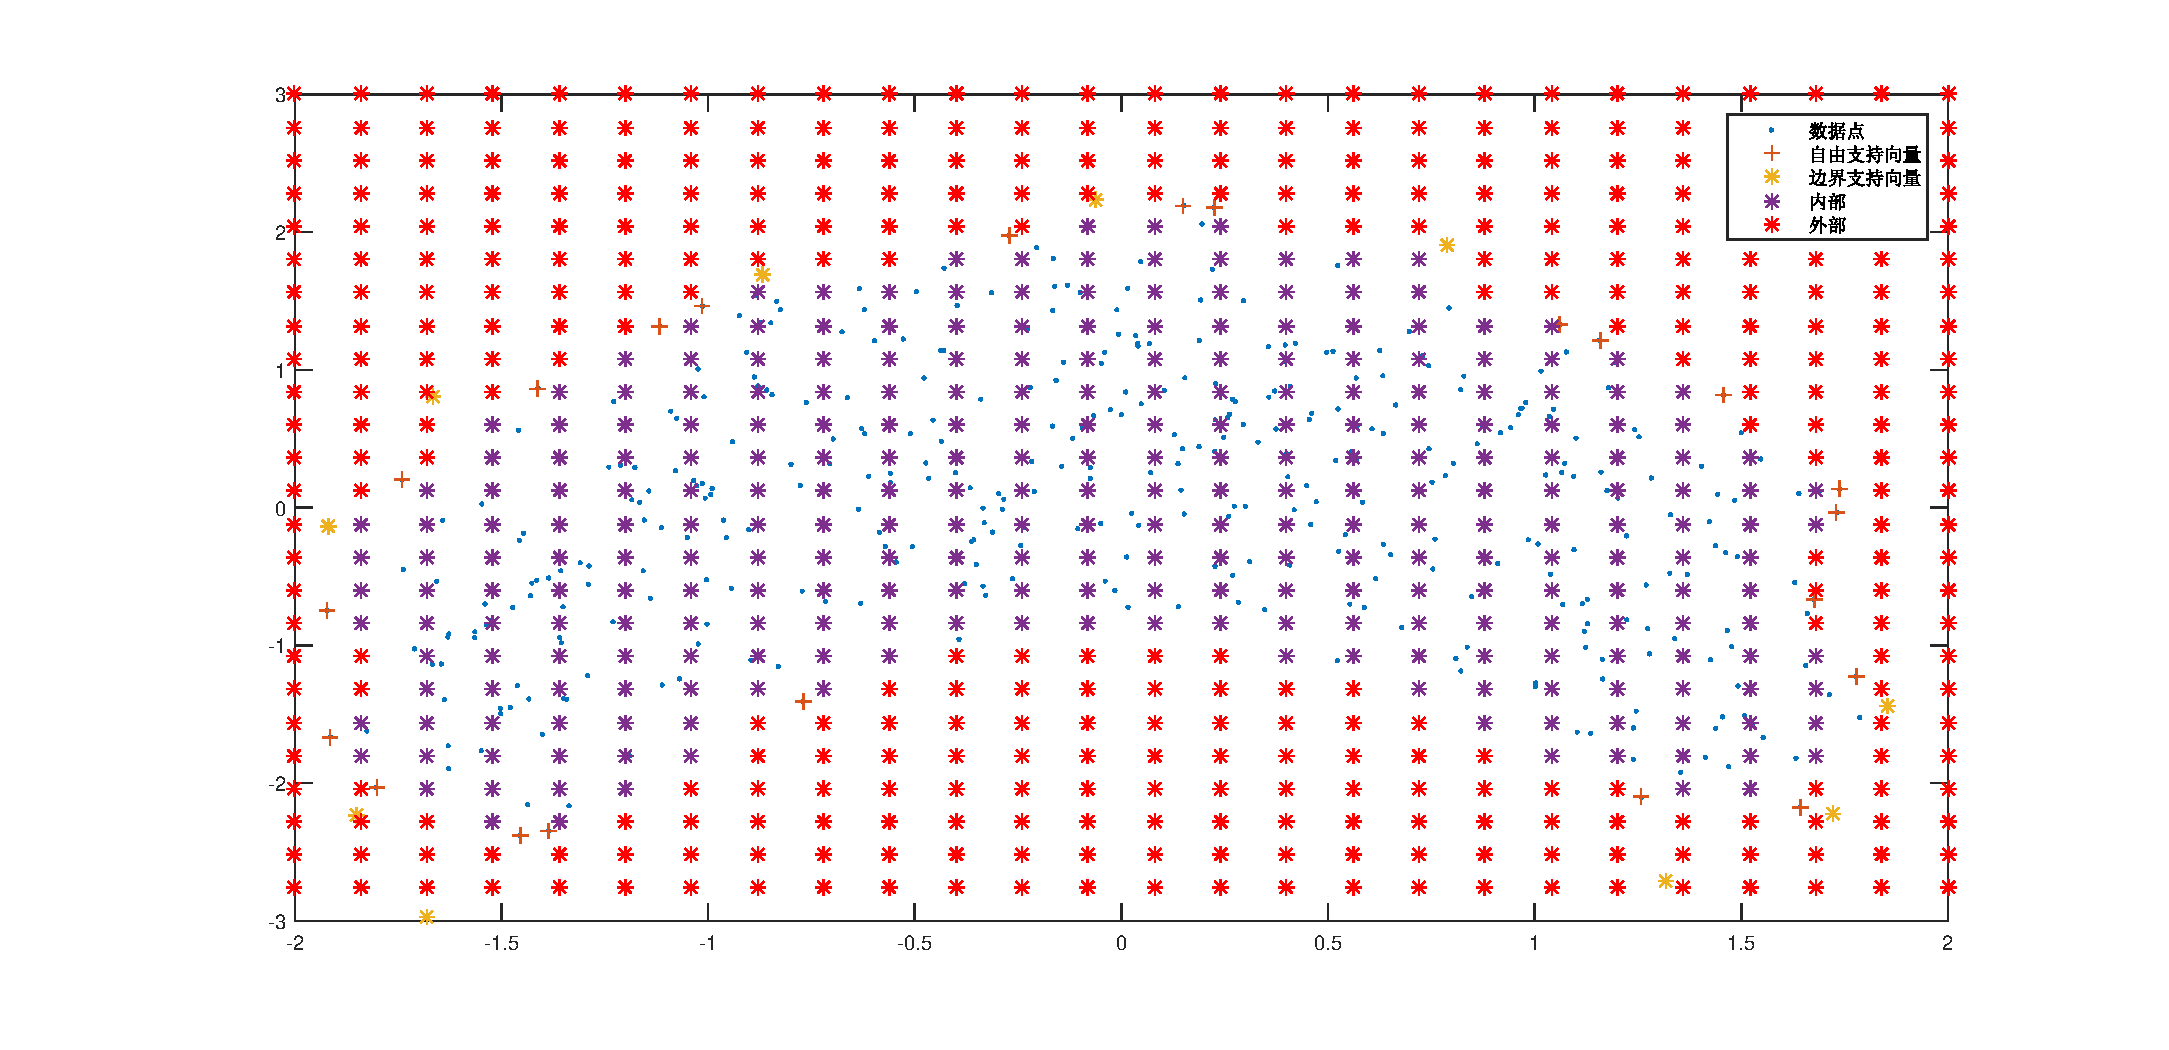
\includegraphics[width = 5in]{banana.eps}
\end{center}


\subsubsection{灵敏度分析}
我们选取了一组数据进行灵敏度分析测试,即随着参数的改变,算法的表现如何.

对于大肠杆菌数据集,我们让C增加,观察准确率,召回率,和准确度率的变化.

准确率的变化:


\begin{center}
\includegraphics[width = 4in]{precision.eps}
\end{center}

召回率的变化:

\begin{center}
\includegraphics[width = 4in]{recall.eps}
\end{center}

精确度的变化:


\begin{center}
\includegraphics[width = 4in]{prec.eps}
\end{center}


由此课件,增加C会增加超球的半径,于是引入一些假阳性,消除了一些假阴性,导致准确率变低,召回率略微上升,精确度也只是略微变低,但不明显。


随着$\sigma$变大,超球会变得更加光滑,于是支持向量的数量变少。如图所示:
\begin{center}
\includegraphics[width = 4in]{shit.pdf}
\end{center}



\section{小结}

\subsection{成员分工}

任亮亮同学负责公式的推导,两位同学共同完成了文献的阅读,两位同学共同完成了代码的书写与调试,夏斐同学完成了数据的测试,报告由两位同学共同完成。

\subsection{感想与体会}

在这次运筹大作业的过程中,我们学会了用优化的方法解决了实际问题。优化在机器学习中有广泛的应用,SMO只是其中的冰山一角,还有更多有意思的算法会用到优化的知识。我们感受到在这次大作业中学到很多。


\section{参考文献}
\begin{enumerate}
\item Bottou, Léon, and Chih-Jen Lin. "Support vector machine solvers." Large scale kernel machines (2007): 301-320.
APA	

\item Tax, David MJ, and Robert PW Duin. "Support vector data description." Machine learning 54.1 (2004): 45-66.

\item Bache, K., Lichman, M.: UCI machine learning repository (2013). 

\end{enumerate}


\end{CJK}



\end{document}